\documentclass[10pt,landscape]{article}
\usepackage{multicol}
\usepackage{graphicx}
\usepackage{calc}
\usepackage{ifthen}
\usepackage{color}
\usepackage[landscape]{geometry}

\ifthenelse{\lengthtest { \paperwidth = 11in}}
	{ \geometry{top=.05in,left=.2in,right=0in,bottom=.05in} }
	{\ifthenelse{ \lengthtest{ \paperwidth = 297mm}}
		{\geometry{top=1cm,left=1cm,right=1cm,bottom=1cm} }
		{\geometry{top=1cm,left=1cm,right=1cm,bottom=1cm} }
	}

% Turn off header and footer
\pagestyle{empty}
 

% Redefine section commands to use less space
\makeatletter
\renewcommand{\section}{\@startsection{section}{1}{0mm}%
                                {-1ex plus -.5ex minus -.2ex}%
                                {0.5ex plus .2ex}%x
                                {\normalfont\large\bfseries}}
\renewcommand{\subsection}{\@startsection{subsection}{2}{0mm}%
                                {-1explus -.5ex minus -.2ex}%
                                {0.5ex plus .2ex}%
                                {\normalfont\normalsize\bfseries}}
\renewcommand{\subsubsection}{\@startsection{subsubsection}{3}{0mm}%
                                {-1ex plus -.5ex minus -.2ex}%
                                {1ex plus .2ex}%
                                {\normalfont\small\bfseries}}
\makeatother

% Define BibTeX command
\def\BibTeX{{\rm B\kern-.05em{\sc i\kern-.025em b}\kern-.08em
    T\kern-.1667em\lower.7ex\hbox{E}\kern-.125emX}}

% Don't print section numbers
\setcounter{secnumdepth}{0}


\setlength{\parindent}{0pt}
\setlength{\parskip}{0pt plus 0.5ex}


\newlength{\MyLen}
\settowidth{\MyLen}{\texttt{letterpaper}/\texttt{a4paper} \ }
% -----------------------------------------------------------------------

\begin{document}

\raggedright
\footnotesize
\begin{multicols}{3}

\setlength{\premulticols}{1pt}
\setlength{\postmulticols}{1pt}
\setlength{\multicolsep}{1pt}
\setlength{\columnsep}{2pt}

\begin{center}
\includegraphics[width=198.5px]{header.png}\end{center}

\section{Standard navigation keys}
A variety of standard emacs/readline navigation keys have analogs
throughout emergent. The first line of each top-level section lists
which of these work there. On OSX you can swap the Cmd and Ctrl keys
and Cmd+V is paste while Ctrl+V is Page Down. \\
\begin{tabular}{@{}ll@{}}
\\
\verb!Tab/Shift+Tab! & Forward/Backwards through elements/interface \\
\verb!Page Up/Down!    & Move cursor to the top/bottom or first/last element\\
\verb!Ctrl+Space!    & Enable select as you navigate mode. \\
\verb!Ctrl+F!    & Move cursor forwards or expand node. \\
\verb!Ctrl+B!    & Move cursor backwards or expand node. \\
\verb!Ctrl+N!    & Move cursor down one line. \\
\verb!Ctrl+P!    & Move cursor up one line. \\
\verb!Ctrl+A!    & Move cursor to first character \\
\verb!Ctrl+E!    & Move cursor to last character \\
\verb!Ctrl+D!  & Delete item in focus or all selected items. \\
\verb!Ctrl+G!  & Deselect text or tree selection. \\
\verb!Ctrl+X/W! & Cut. \\
\verb!Ctrl+C/Alt+W! & Copy. \\
\verb!Ctrl+V/Y! & Paste.
\end{tabular}

\section{Global project}
\begin{tabular}{@{}ll@{}}
\verb!Standard!    & Tab \\
\verb!Ctrl+S!    & Save project. \\
\verb!Ctrl+left! & Backwards in navigation history \\
\verb!Ctrl+right! & Forwards in navigation history \\
\verb!F5!  & Refresh GUI. \\
\verb!Ctrl/Alt+J! & Move global focus left \\
\verb!Ctrl/Alt+L! & Move global focus right
\end{tabular}

\section{Project tree and program tree}
\settowidth{\MyLen}{\texttt{multicol} }
\begin{tabular}{@{}ll@{}} \\
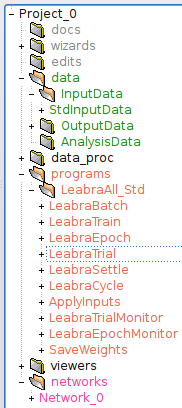
\includegraphics[width=91px]{treebrowser.png}   & 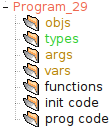
\includegraphics[width=150px]{programcode.png}
\end{tabular}
\begin{tabular}{@{}ll@{}}
\verb!Standard!    & Page,Ctrl+Space/F/B/N/P/D/G/X/W/C/V/Y. \\
\verb!Any 1-3 chars!    & Find as you type. Moves cursor to next matching line. \\
\verb!Ctrl+I!    & New item below cursor. \\
\verb!Alt+F!  & Find from selected node. \\
\verb!Ctrl+M!  & Duplicate element(s).
\end{tabular}

\subsection{New elements in project tree}
\begin{tabular}{@{}ll@{}}
\verb!do Ctrl+I!    & New Doc \\
\verb!da Ctrl+I!    & New DataTable \\
\verb!la Ctrl+I!    & New Layer \\
\verb!P Ctrl+I!    & New Project \\
\verb!pr Ctrl+I!    & New Program \\
\verb!n Ctrl+I!    & New Network \\
\verb!sp Ctrl+I!    & New Spec
\end{tabular}

\subsection{New elements in program tree}
These sequences insert new items. Press Ctrl+left,left afterwards to navigate back to where you were. \\
\begin{tabular}{@{}ll@{}}
\verb!obj Ctrl+I Type!    & New obj of Type \\
\verb!var Ctrl+I!    & New var \\
\verb!arg Ctrl+I!    & New arg \\
\verb!fun Ctrl+I!    & New fun \\
\verb!init Ctrl+I Name!    & New init code Name \\
\verb!prog Ctrl+I Name!    & New prog code Name
\end{tabular}

\section{css console and text fields}
\begin{tabular}{@{}ll@{}}
\verb!Standard!  & Ctrl+F/B/N/P/A/E/D/X/W/C/V/Y. \\
\verb!Ctrl+K! & Kill text until end of line. \\
\verb!Ctrl+right! & Move cursor one word forward. \\
\verb!Ctrl+left! & Move cursor one word backwards. \\
\verb!Ctrl+shift+right! & Highlight one word forward. \\
\verb!Ctrl+shift+left! & Highlight one word backwards.
\end{tabular}

\subsection{css console}
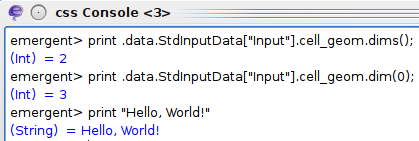
\includegraphics[width=209.5px]{console.png} \\
\begin{tabular}{@{}ll@{}}
\verb!Ctrl+L!    & Clear console buffer history. \\
\verb!Ctrl+L!    & Delete highlighted text.
\end{tabular}

\subsection{Text fields}

\includegraphics[width=205px]{path.png} \\
\begin{tabular}{@{}ll@{}}
\verb!Ctrl+L!    & Text completion lookup.  \\
\verb!Ctrl+U!    & Highlight all.
\end{tabular} 

\section{Help Browser}
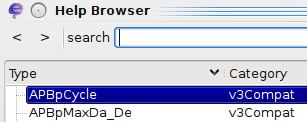
\includegraphics[width=240px]{helpbrowser.png}
\begin{tabular}{@{}ll@{}}
\verb!Standard!  & Tab,Page,Ctrl+F/B/N/P/A/E/X/W/C/V/Y. \\
\verb!F1!  & Help Browser. \\
\verb!Ctrl+S!  & Toggle Search/Find focus. \\
\end{tabular}

\section{DataTables and matrices}
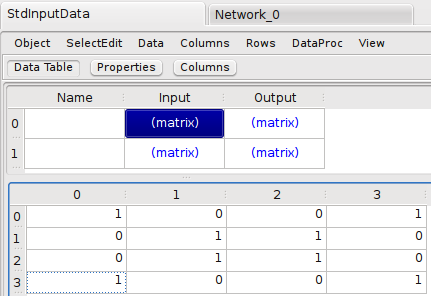
\includegraphics[width=215.5px]{datatable.png}
\begin{tabular}{@{}ll@{}}
\verb!Standard!  & Page,Ctrl+F/B/N/P/A/E/C/V/D/G/Y. \\
\verb!Ctrl+T!    & Switch between table and matrix focus. \\
\verb!Ctrl+I!    & Insert new row. \\
\verb!Ctrl+M!    & Duplicate row. \\
\verb!Ctrl+Space!    & Start editing cell.
\end{tabular}

\section{Edit panels}
See the ``Text fields'' section for shortcuts that work on the text
fields of edit panels.
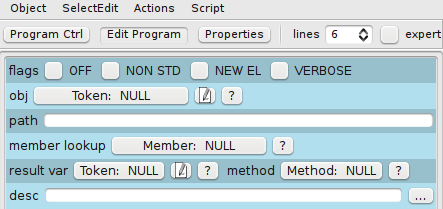
\includegraphics[width=221.5px]{middlepanel.png}
\\ \settowidth{\MyLen}{\texttt{multicol} }
\begin{tabular}{@{}ll@{}} \\
\verb!Standard!    & Tab  \\
\verb!Up/Down arrow!    & (numeric field) Increase/decrease value. \\
\verb!Up/Down arrow!    & (dropdown) Move up/down. \\
\verb!ESC!    & Revert changes. \\
\verb!Ctrl+Enter!    & Apply changes. \\
\verb!Space!    & Open token chooser and Check/uncheck flag.\\
\verb!Ctrl+L!    & (expression fields) Lookup information.
\end{tabular}

\section{Choosers}
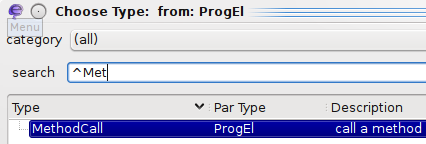
\includegraphics[width=213px]{progel.png} \\
\begin{tabular}{@{}ll@{}}
\verb!Standard!  & Tab,Ctrl+F/B/N/P/A/E/D/X/W/C/V/Y.
\end{tabular}

\section{Docs}
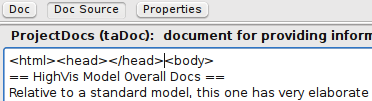
\includegraphics[width=186px]{doc.png} \\
\begin{tabular}{@{}ll@{}}
\verb!Standard!  & Tab,Space,Ctrl+F/B/N/P/A/E/D/X/W/C/V/Y.
\end{tabular}


\end{multicols}

\end{document}
